\documentclass{article}

\usepackage[a4paper,margin=2cm]{geometry}
\usepackage{color, soul}
\usepackage{titlesec}
\usepackage{enumitem}
\usepackage{pdfpages}
\usepackage{multicol}
\usepackage{fancyvrb}
\usepackage{float}

\title{SWEN30006 Assignment 2 - Report}
\date{\today}
\author{Workshop 09, Team 02\\Lucas Fern \& Cameron Maddern}

\begin{document}
\maketitle
This project required changes to be made to an existing Cribbage card game trainer system to add scoring and logging functionality. These additions were made with the use of a variety of design patterns in order to have minimum impact on the existing code, and therefore reduce coupling between existing classes and classes added for the new functionality.\\[2mm]
This report will discuss the changes which have been made, provide justification for the design patterns used, and argue in favour of these design patterns over the use of others where appropriate. The additional classes will be covered first, then how these additional classes were integrated into the existing system.\\[2mm]
A class diagram of the updated design is included at the end of the report and will be relevant to visualise all changes to the system. 

\section{Cribbage Observers}
In an effort to minimise coupling between added classes and maximise cohesion within them, a \verb|CribbageObserver| interface was implemented. This allowed classes to subscribe to various events of the Cribbage game, and respond with unique actions. This required the addition of a list of subscribers in the main \verb|Cribbage| class, as well as a method to register new subscribers.

\subsection{Cribbage Events}
\label{sec: crib events}
Now that a publish-subscribe pattern is implemented it must be decided when events are broadcast to the subscribers. There are a variety of events in the game of Cribbage, and it was decided that all events which relate to the logging and scoring functionality will be broadcast to the subscribers. This allows - for example - the logging functionality for the \verb|deal| to be implemented by an observer responding to a \verb|Deal| event. The various subscribers to Cribbage Events are discussed further in Section \ref{sec: crib subscribers}.\\[2mm]
The complete list of \verb|CribbageEvent|s implemented appears on the right side of the class diagram, and their functionality is briefly summarised below:
\begin{multicols}{2}
    \begin{itemize}
        \item \verb|SetSeed|\\[2mm]
        Subscribers are notified of this event when the game's seed is set from the \verb|cribbage.properties| file. The event contains the random seed which was chosen.
        \item \verb|InitPlayer|\\[2mm]
        This event is broadcast when the players of the game are initialised and assigned a number. This provides subscribers with information about the player type which has been initialised (\textit{eg.} \verb|cribbage.RandomPlayer|) and their number.
        \item \verb|Discard|\\[2mm]
        This event is created once for each player each game, when the player has selected which cards to discard. It provides observers with the players number, and a \verb|jcardgame.Hand| object containing the cards they selected for discarding.
        \item \verb|PlayStarter|\\[2mm]
        The \verb|PlayStarter| event is published once per game when the starter card is selected, and provides the starter card as a \verb|jcardgame.Card|.
        \item \verb|Play|\\[2mm]
        This event is raised on every turn of the game, when a player selects the card they wish to play. It contains the player's number, the card they played, and the total face value of the current board after adding this card.
        \item \verb|Show|\\[2mm]
        The \verb|Show| event occurs at the end of the game when play has ceased and players are showing card combinations from their hands to be scored. This event contains information about the player's number, the starter card, and the cards that they are showing to be scored.
    \end{itemize}
\end{multicols}
\begin{itemize}
    \item \verb|Score|\\[2mm]
    The \verb|Score| event is a special type of event raised by the Cribbage Scorer in response to other events, it occurs whenever a player's score is incremented, and contains data on the amount of points scored, their total score, and the type of score achieved. This will be discussed further in \ref{sec: crib scorer}.
\end{itemize}
Each of these events also overrides the default \verb|toString()| method. Their implementation of the method returns a \verb|String|, formatted as required for the logging functionality. This will be discussed further in Section \ref{sec: crib logger}


\subsection{Cribbage Subscribers}
\label{sec: crib subscribers}
Subscribers are classes which implement the \verb|CribbageObserver| interface and register with the \verb|Cribbage| class to be notified of game events. Their creation and registration is done inside the \verb|Cribbage| class since currently the only subscribers are the Logger and Scorer, which was not complex enough to justify their creation in an external factory.
\subsubsection{Cribbage Scorer}
\label{sec: crib scorer}
The \verb|CribbageScorer| is a singleton class which is cohesively responsible for handling all scoring events in the Cribbage game. \verb|CribbageScorer| subscribes to the \verb|Cribbage| class and its \verb|update()| method is called whenever an event (defined in Section \ref{sec: crib events}) occurs.\\[2mm]
When an event is received, the \verb|CribbageScorer| updates its records of the moves in the game and delegates responsibility for the scoring of events out to individual score handling classes, which each implement the logic for a single method of earning points. Since there are many scoring methods, these are instantiated by a \verb|ScorerFactory| when the \verb|CribbageScorer| is created. The score handling classes are discussed below.

\paragraph{Score Handlers} implement the \verb|ScoringEvent| interface, which requires that they define the following methods:
\begin{figure}[H]
\centering
\begin{BVerbatim}
int scoreForPlay(Hand cardSet, int playerScore, int playerNum);
int scoreForShow(Hand cardSet, int playerScore, int playerNum);
\end{BVerbatim}
\end{figure}
\noindent The distinction between the two methods \verb|scoreForPlay()| and \verb|scoreForShow()| allows for variations in scoring to be easily implemented, since there certain behavioural differences between scoring events during and after the Play stage of the game. For example, flushes are only relevant in the show stage, so do not calculate a score in their \verb|scoreForPlay()| method.\\[2mm]
This design also allows for more complex variations, for example, if an alternative ruleset did not include flushes then this would be implemented by not subscribing the \verb|HandleFlushes| class to the \verb|CribbageScorer|, or if a variation were to not include runs in the Show phase of the game, then \verb|scoreForShow()| in the \verb|HandleRuns| class could simply return the \verb|playerScore| that was passed in.\\[2mm]
The complete list of \verb|ScoringEvent|s implemented appears on the bottom left side of the class diagram, and their functionality is briefly summarised below:
\begin{multicols}{2}
    \begin{itemize}
        \item \verb|HandleTotals|\\[2mm]
        This \verb|ScoringEvent| determines points allocated for any combinations of cards who's scores sum to 15 as well as for when total face values reach 15 or 31. The amount of points allocated for this is customisable with the \verb|POINTS_FOR_TOTALS| constant.
        \item \verb|HandleFlushes|\\[2mm]
        This \verb|ScoringEvent| determines points allocated for any combination of 4 or 5 cards of the same suit shown in the Show phase. Its \verb|scoreForPlay()| method is unimplemented.
        \item \verb|HandlePairs|\\[2mm]
        This \verb|ScoringEvent| determines points allocated for any pair, triple, or 4-of-a-kind. Points allocated for pairs of varied sizes can be adjusted with the \verb|PAIR_SCORE|, \verb|TRIP_SCORE| and \verb|QUAD_SCORE| constants.
        \item \verb|HandleRuns|\\[2mm]
        This \verb|ScoringEvent| determines points allocated for runs of cards, accounting for run sizes from \verb|SHORTEST_RUN| to \verb|min(LONGEST_RUN, handCards.size())| where \verb|handCards| is the card set from which runs are being searched for. This ensures the program does not search for a run greater than the amount of cards available in the given hand.
        \item \verb|HandleStarters|\\[2mm]
        This \verb|ScoringEvent| determines points allocated for the \verb|dealer| if the first card is a Jack as well as finding any scores from Jacks during the show phase.
    \end{itemize}
\end{multicols}
\noindent This design allows for simple extensibility as any new method of scoring can simply be defined as a new class inheriting the \verb|ScoringEvent| interface, and once it is added to the \verb|ScorerFactory| it will be interrogated for score updates after each Play and Show event.\\[2mm]
Finally, the logging functionality for scores is enabled by each of the \verb|ScoringEvent|s. Once the amount of points scored by an event is determined, the score handler is able to access the singleton \verb|CribbageLogger| instance and provide it with a \verb|new Score| event. By creating a score event with all the required logging information the remaining logging behaviour is all handled inside the \verb|CribbageLogger| class and thus cohesion within the \verb|ScoringEvents| is maximised. The internal behaviour of the \verb|CribbageLogger| will be discussed in detail below.

\subsubsection{Cribbage Logger}
\label{sec: crib logger}
The \verb|CribbageLogger| is a singleton class, which appears in the bottom left of the class diagram and is cohesively responsible for all of the logging functionality of the game. As a subscriber to the \verb|Cribbage| class, the logger's \verb|update()| method is called whenever an event (defined in Section \ref{sec: crib events}) occurs. The event is passed through to the class in this method call.\\[2mm]
On notification of any event, the cribbage logger calls the event's \verb|toString()| method, yielding the information required for logging, and uses a \verb|BufferedWriter| to write this to \verb|cribbage.log|. Taking a \verb|Play| event for example, the contents and respective string representation might be:
\begin{figure}[H]
\centering
\begin{BVerbatim}
examplePlay = {                              |
    eventId: "play",  [String]               |
    playerId: "P0",   [String]               |      String representation:
    totalPoints: 23,  [int]                  |      "play,P0,23,KH"
    card: KH          [jcardgame.Card]       |  
}                                            |
\end{BVerbatim}
\end{figure}
\noindent This highly cohesive design, enabled by the observer pattern, is all that is required for the logging functionality.

\section{Changes to Existing Classes}
Changing existing classes was avoided as much as possible when adding the new functionality to reduce the possibility of bloated classes, and reduce coupling with new classes. This section will provide justification for the few changes which were made to the existing classes despite these considerations.
\subsection{Cribbage}
The \verb|Cribbage| class is where most of the changes to existing classes were made. The changes made here are:
\begin{itemize}
    \item \textbf{Adding the Subscriber Functionality}\\[2mm]
    Since the majority of additions to the system were made by implementing the observer pattern, an attribute had to be added to the \verb|Cribbage| class to store the list of classes which subscribe to the events. A method to register subscribers was also added so that the \verb|CribbageScorer| and \verb|CribbageLogger| could register themselves to be notified.
    \item \textbf{The Registration of Subscribers}\\[2mm]
    Since they are separate classes, the \verb|CribbageScorer| and \verb|CribbageLogger| must be instantiated at the beginning of the game, and registered as subscribers to the \verb|Cribbage| class. It was decided that this was an appropriate amount of code (2 lines) to add to the cribbage class, as opposed to creating a factory to instantiate these classes (which would itself need to be initialised on start-up.)
    \item \textbf{Privacy / Visibility Changes}\\[2mm] 
    To support the functionality of the new system, it was sensible to change the privacy of certain methods. The most significant change was to each of the 4 \verb|canonical()| methods, which were \verb|private| instance methods in the original design, and have been changed to \verb|public| \verb|static| methods. They were able to be converted to \verb|static| since the conversion of \verb|jcardgame| objects to \verb|String|s did not strictly require any attributes of the \verb|Cribbage| instance.\\[2mm]
    This change was made to support the logging functionality, since the log file contains canonical representations of the cards and hands, and the \verb|String|ification of the \verb|jcardgame| objects occurs in the \verb|toString()| methods of each of the \verb|CribbageEvent|s. Considering the alternative would be to pass string representations as well as the original \verb|jcardgame| objects around with each event; and the fact that there is no clear downside to this change, this was an obvious choice.
\end{itemize}

\section{Consideration of Alternative Designs}
The final design presented in this report was the product of many design iterations. Originally, designs with high coupling to the \verb|Cribbage| class were considered as alternatives to the final design, which is centred around the implementation of the Observer pattern. These alternative implementations would have involved creating Logging and Scoring classes and calling these directly from the \verb|Cribbage| class when relevant events occurred in the game. This clearly causes enormous coupling between the classes since logging and scoring functionality are complex and required at all stages of the game.\\[2mm]
The final design is the antithesis of this highly coupled design, and was chosen for its implementation requiring extremely small changes to existing classes - these being the notifications to subscribers of new events. This design ultimately allows for so much extensibility that future editions of the game - such as an update of the GUI - could subscribe to the events raised by the observer pattern to conduct a variety of other operations (again such as updating GUI elements).\\[2mm]
Alternatives were also considered to the implementation of the scoring method. Originally the score handling was done in methods of the \verb|ScoreHandler| class, but it was clear that the complexity of scoring rules and potential for extensibility made it a sensible design decision to extract each scoring rule into its own class and instantiate these within a factory.\\[2mm]
Again, all of these design decisions and their integration with the existing system can be visualised with the help of the design class diagram on the following page.

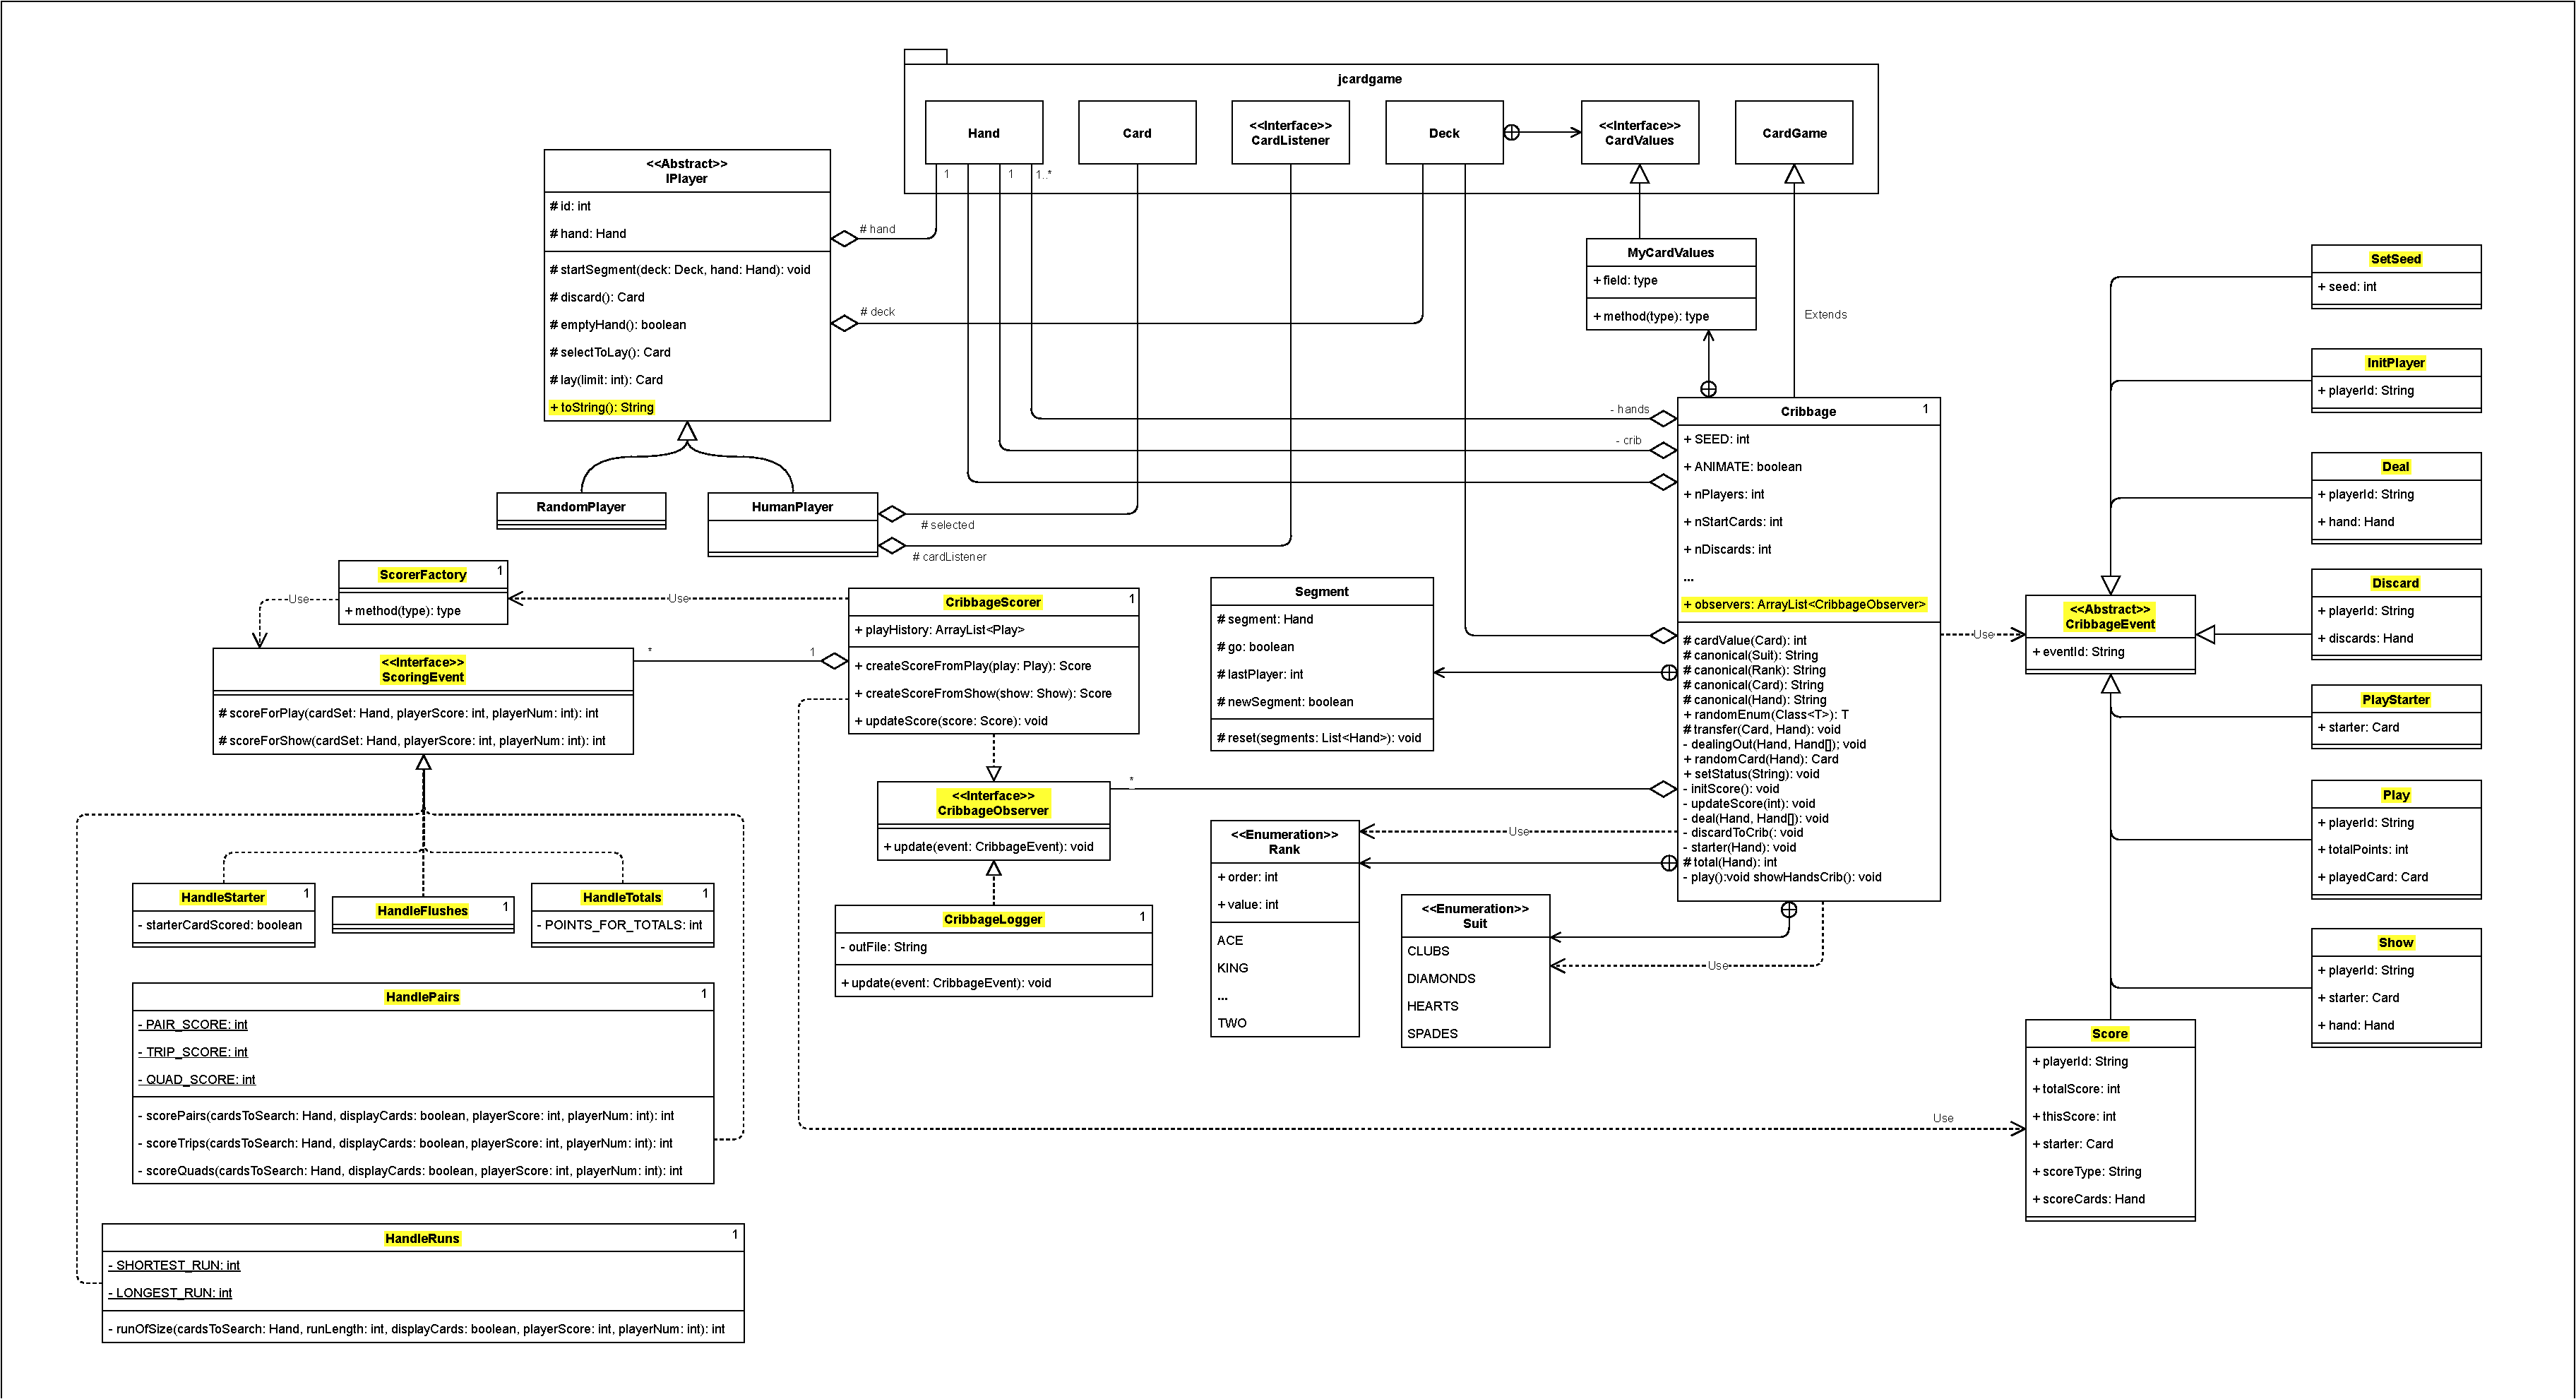
\includepdf[pages=1, fitpaper=true]{design-class-diag.pdf}
\end{document}
